\documentclass[presentation]{beamer}

\usepackage{tikz}
\usetikzlibrary{positioning,calc}
\usetikzlibrary{shapes.geometric}
\usetikzlibrary{backgrounds}% only to show the bounding box
\usetikzlibrary{shapes,arrows}
\usepackage{pgfplots}
\usepackage{pgfplotstable}
\usetikzlibrary{pgfplots.groupplots}
\pgfplotsset{compat=1.12}
\usepackage{appendixnumberbeamer}
\usepackage{amsmath}
\date{27th March 2017}
\usetheme{firedrake}

\pgfplotscreateplotcyclelist{decent cycle}{%
  {blue, mark=*, mark options={fill=blue},
    mark size=2pt},
  {cyan, mark=square*, mark options={fill=cyan},
    mark size=2pt},
  {magenta, mark=triangle*, mark options={fill=magenta},
    mark size=3pt},
  {blue, mark=*, mark options={fill=blue},
    mark size=2pt},
  {cyan, mark=square*, mark options={fill=cyan},
    mark size=2pt},
  {magenta, mark=triangle*, mark options={fill=magenta},
    mark size=3pt},
}

\pgfplotsset{
  decent/.style={
    cycle list name=decent cycle,
  }
}
\renewcommand{\vec}[1]{\ensuremath{\boldsymbol{#1}}}
\newcommand{\ddt}[1]{\frac{\partial #1}{\partial t}}
\newcommand{\zhat}{\hat{\vec{z}}}
\newcommand{\W}{\ensuremath{\mathbb{W}}}

\DeclareMathOperator{\grad}{grad}
\let\div\relax
\DeclareMathOperator{\div}{div}
\DeclareMathOperator{\curl}{curl}

\newcommand{\inner}[1]{\left\langle #1 \right \rangle}

\newcommand{\KSP}[2]{\ensuremath{\mathcal{K}\left(#1, \mathbb{#2}\right)}}
\newcommand{\ksp}[1]{\KSP{#1}{#1}}

\newcommand{\highlight}[1]{\colorbox{red!20}{\color{black} #1}}

\author{Lawrence Mitchell\inst{1,*}}
\institute{
\inst{1}Departments of Computing and Mathematics, Imperial College
London

\inst{*}\texttt{lawrence.mitchell@imperial.ac.uk}
}

\graphicspath{{./\jobname.figures/}}

\newcommand{\arxivlink}[2]{%
  \href{http://www.arxiv.org/abs/#1}%
  {{\small\texttt{arXiv:\,#1\,[#2]}}}%
}
\newcommand{\doilink}[1]{%
  \href{http://dx.doi.org/#1}%
  {{\small\texttt{doi:\,#1}{}}}%
}
\usepackage[url=false,
            doi=true,
            isbn=false,
            style=authoryear,
            firstinits=true,
            uniquename=init,
            backend=biber]{biblatex}

\setbeamertemplate{bibliography item}{}
\renewcommand{\bibfont}{\footnotesize}
\addbibresource{references.bib}

\setlength{\bibitemsep}{1ex}
\setlength{\fboxsep}{1pt}

\renewbibmacro{in:}{}
\DeclareFieldFormat[article]{volume}{\textbf{#1}}
\DeclareFieldFormat{doi}{%
  doi\addcolon%
  {\scriptsize\ifhyperref{\href{http://dx.doi.org/#1}{\nolinkurl{#1}}}
    {\nolinkurl{#1}}}}
\AtEveryBibitem{%
\clearfield{pages}%
\clearfield{issue}%
\clearfield{number}%
}

\usepackage{minted}
\RecustomVerbatimEnvironment{Verbatim}{BVerbatim}{}
\title{Specifying and solving PDEs}
\subtitle{\only<1>{\phantom{$\dots$ easily?}}\only<2>{$\dots$ easily?}}

\begin{document}

\maketitle

\section{Introduction}

\begin{frame}
  \frametitle{Overview}
  Philosophy

  Numerical solution of PDEs using finite elements

  A generative approach

  What did we gain?

  Examples and discussion
\end{frame}

\begin{frame}
  \frametitle{A barrier to progress}
  \begin{lemma}
    Developing sophisticated numerical models ``from scratch'' is a
    lot of work.
  \end{lemma}
  \begin{corollary}
    Many new advances in methods are only tried on simple problems.

    Better numerical methods take a long time to move into ``real
    world'' application domains.
  \end{corollary}
\end{frame}

\begin{frame}
  \frametitle{Why does it happen like this?}
  \begin{itemize}[<+->]
  \item ``I need to solve a PDE''
  \item (search for software that solves my problem)
  \item ``All these libraries are too complicated''
  \item (2 weeks writing code)
  \item ``That was easy''
  \item ``Oh wait, I need parallel/adaptivity/high-order/...''
  \item (3 years writing code)
  \item ``That was easy''
  \end{itemize}

  \begin{uncoverenv}<+>
    We should be able to do better.
  \end{uncoverenv}
\end{frame}

\begin{frame}
  \frametitle{Why are libraries too complicated?}
  \begin{itemize}
  \item Evidence that the \emph{abstraction level} is wrong.
  
  \item If I want to solve a PDE, in the first instance, I don't (or
    shouldn't) care about parallel computing.
  
  \item Well-designed abstractions present low barrier to entry, without
    only being useful for toy problems.

  \item Then, we can build on them, rather than starting from scratch
    every time.
  \end{itemize}
\end{frame}

\begin{frame}[fragile, t]
  \frametitle{In the beginning}
  Compute $y \leftarrow \nabla^2 x$ using finite differences.
  \begin{equation*}
    y_{i,j} = x_{i-1, j} + x_{i+1, j} + x_{i, j-1} + x_{i, j+1} - 4x_{i,j}    
  \end{equation*}

  \begin{onlyenv}<2>
    \begin{block}{Before 1953}
\begin{minted}[fontsize=\tiny]{asm}
        ...
        faddp   %st, %st(1)
        movl    -8(%ebp), %edx
        movl    %edx, %eax
        sall    $2, %eax
        addl    %edx, %eax
        leal    0(,%eax,4), %edx
        addl    %edx, %eax
        sall    $2, %eax
        movl    %eax, %edx
        movl    -4(%ebp), %eax
        addl    %edx, %eax
        subl    $101, %eax
        flds    x.3305(,%eax,4)
        flds    .LC0
        fmulp   %st, %st(1)
        faddp   %st, %st(1)
        fstps   y.3307(,%ecx,4)
        ...
\end{minted}
    \end{block}
  \end{onlyenv}
  \begin{onlyenv}<3->
    \begin{block}{After 1953}
\begin{minted}[fontsize=\tiny]{fortran}
      PROGRAM MAIN
      PARAMETER (N=100)
      REAL X(N,N), Y(N,N)
      DO 10 J=2,N-1
         DO 20 I=2,N-1
            Y(I,J)=X(I-1,J)+X(I+1,J)+X(I,J-1)+X(I,J+1)+4*X(I,J)
 20      CONTINUE
 10   CONTINUE
      DO 30 I=1,N
         Y(I,1) = 0.0
         Y(I,N) = 0.0
         Y(1,I) = 0.0
         Y(N,I) = 0.0
 30   CONTINUE
      END
\end{minted}
    \end{block}
  \end{onlyenv}
\end{frame}

\begin{frame}
  \begin{block}{Pros}
    \begin{itemize}
    \item Not tied to a particular piece of hardware
    \item Easier to understand
    \item Composable
    \end{itemize}
  \end{block}
  \begin{block}{Cons}
    \begin{itemize}
    \item Lost full control over program execution
    \item Compiler may do a bad job optimising
    \end{itemize}
  \end{block}
\end{frame}

\begin{frame}[standout]
  Describe, don't implement
\end{frame}

\section{Solving PDEs}

\begin{frame}[allowframebreaks]
  \frametitle{Finite element crash course}
  \begin{align*}
    F(u) &= 0 \text{ in $\Omega$}\\
    u &= g \text{ on $\Gamma_1$}\\
    \frac{\partial u}{\partial n} &= h \text{ on $\Gamma_2$}
  \end{align*}
  Seek \emph{weak} solution in some space of functions $V(\Omega)$.

  Find $u\in V$ s.t.
\begin{equation*}
\int_\Omega \!F(u) v\, \text{d}x = 0 \quad \forall\, v \in V
\end{equation*}
Choose discrete $V_h \subset V$, and seek $u_h \in V_h$.

Pick \emph{basis} for $V_h$ with finite support.

\pagebreak
Divide domain $\Omega$ into triangulation $\mathcal{T}$.

Integrals become sum over element integrals
\begin{equation*}
  \int_\Omega\! F(u_h) v_h \, \text{d}x =
  \sum_{e \in \mathcal{T}} \int_e\! F(u_h)v_h\, \text{d}x
\end{equation*}

Perform element integrals with numerical quadrature
\begin{equation*}
  \int_e F(u_h)v_h\,\text{d}x = \sum_q w_q F(u_h(q)) v_h(q)\,\text{d}x
\end{equation*}

$F(u_h(q))$ is ``user-specified''.  Variability in innermost loop.
\end{frame}

\begin{frame}
  \frametitle{Added complexity}
  Compared to the simple finite difference code, I need much more code

  \begin{itemize}
  \item Numerical quadrature
  \item Orthogonal polynomials
  \item Indirections from elements to data
  \end{itemize}

  I can't fit the action of the Laplacian on a slide any more.
\end{frame}

\begin{frame}
  \frametitle{What about solving PDEs}
  \emph{Simple} finite difference models can be programmed from scratch.

  No-one should attempt to write a finite element model from
  scratch. Pick a library:
  \begin{center}
    \small
    \begin{tabular}{lr}
      deal.II   & \url{www.dealii.org}            \\
      DUNE      & \url{www.dune-project.org}      \\
      Firedrake & \url{www.firedrakeproject.org}  \\
      FEniCS    & \url{www.fenicsproject.org}     \\
      FreeFEM++ & \url{www.freefem.org}           \\
      Feel++    & \url{www.feelpp.org}            \\
      MFEM      & \url{mfem.org}                  \\
      NGSolve   & \url{ngsolve.org}               \\
      oomph-lib & \url{oomph-lib.maths.man.ac.uk} \\
      ...       &                                 \\
    \end{tabular}
  \end{center}
\end{frame}

\begin{frame}
  \frametitle{Computational model}
  Abstract model for computing a finite element
  integral:
  \begin{enumerate}
  \item \emph{gather} from global to local
  \item \emph{compute} on local data
  \item \emph{scatter} from local to global
  \end{enumerate}

  Software libraries provide APIs for each of these steps.
\end{frame}

\begin{frame}[fragile]
  You might write code like this.

\begin{minted}[fontsize=\tiny]{cpp}
template<typename EG, typename LFSU, typename X, typename LFSV, typename M>
void jacobian_volume(const EG& eg, const LFSU& lfsu, const X& x, 
                     const LFSV& lfsv, M& mat) const {
  const auto geo = eg.geometry();
  const auto S = geo.jacobianInverseTransposed(qp);
  RF factor = weight*geo.integrationElement(qp);
  double grad[dim][n] = {{0.0}};
  for (int i=0; i<dim; i++)
    for (int k=0; k<dim; k++)
      for (int j=0; j<n; j++)
        grad[i][j] += S[i][k] * gradhat[k][j];
  double A[n][n] = {{0.0}};
  for (int i=0; i<n; i++)
    for (int k=0; k<dim; k++)
      for (int j=0; j<n; j++)
        A[i][j] += grad[k][i]*grad[k][j];
  for (int i=0; i<n; i++)
    for (int j=0; j<n; j++)
      mat.accumulate(lfsu,i,lfsu,j,A[i][j]*factor);
}
\end{minted}
\end{frame}

\begin{frame}
  \begin{block}{Pros}
    \begin{itemize}
    \item Not tied to particular discretisation
    \item Relatively easy to understand
    \item Extensible once code is understood
    \item Free to ``do what you want''
    \end{itemize}
  \end{block}
  \begin{block}{Cons}
    \begin{itemize}
    \item Lost full control over data layout/execution (e.g.
      \texttt{geo.integrationElement(qp)})
    \item Compiler may do a bad job optimising
    \item Need to learn more nouns and verbs
    \item Implementation still tied to numerics
    \end{itemize}
  \end{block}
\end{frame}

\begin{frame}
  \frametitle{Did I implement?}
  \begin{itemize}
  \item \emph{Implementation} details mixed in with numerics
  \item For example, I chose an iteration order.
  \item To change numerics, requires \emph{understanding} the
    low-level implementation.
  \item But, I did have full control over everything going on.
  \end{itemize}
\end{frame}

\begin{frame}[fragile]
  \begin{block}{Assertion}
    Once we pick the discretisation, writing the element integral is mechanical.
  \end{block}
  \begin{corollary}
    Computers are good at mechanical things, why don't we get the
    computer to write the element integral?
  \end{corollary}
\end{frame}

\section{A descriptive approach}

\begin{frame}
  \frametitle{Firedrake}
  An automated finite element system.

  \begin{center}
    \url{www.firedrakeproject.org}\\
    \cite{Rathgeber:2016} \arxivlink{1501.01809}{cs.MS}
  \end{center}

  \begin{itemize}
  \item[IC] Thomas Gibson, David A.~Ham, Mikl\'os Homolya, Lawrence
    Mitchell, {\color{gray}Fabio
    Luporini}, Tianjiao Sun, Paul H.~J.~Kelly
  \item[Bath] Andrew T.~T.~McRae
  \item[\color{gray}ECMWF] \color{gray}Florian Rathgeber
  \item[\color{gray}IBM] \color{gray}Gheorghe-Teodor Bercea
  \end{itemize}
\end{frame}

\begin{frame}
  \frametitle{Exploiting abstractions}
  \begin{itemize}
  \item Firedrake builds on, and extends, embedded DSLs developed in
    the FEniCS project \url{www.fenicsproject.org}
  \item The \emph{Unified Form Language} \parencite{Alnaes:2014} to
    specify variational forms
  \item A symbolic problem description (generic) is woven together with
    problem-specific data, and executed by a runtime Python library
    that does JIT code compilation.
  \end{itemize}
\end{frame}

\begin{frame}[standout]
  Synthesise, don't analyse
\end{frame}

\bgroup
\setbeamertemplate{background}{}
\usebackgroundtemplate{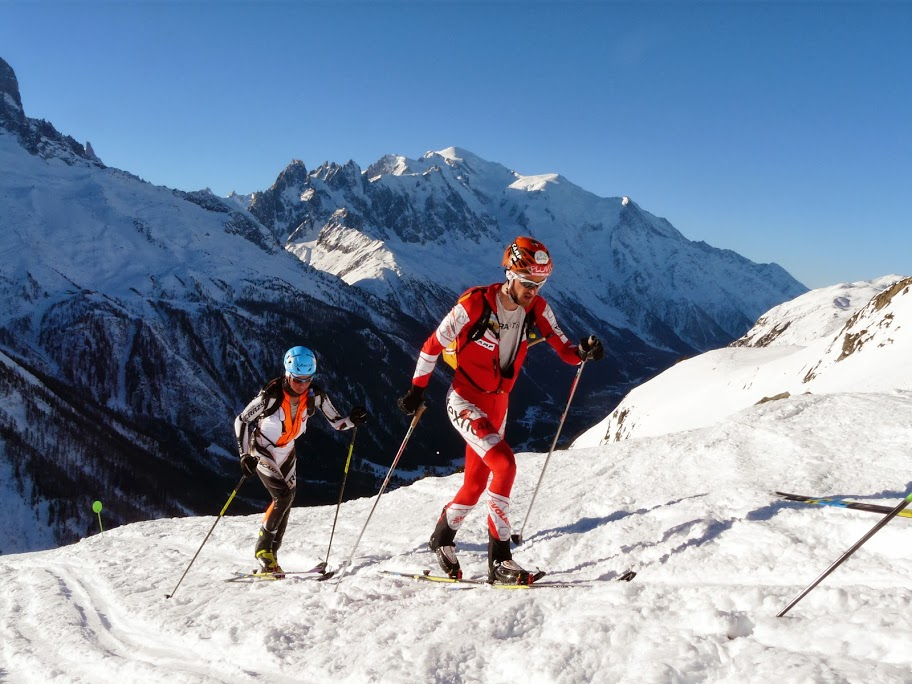
\includegraphics[width=\paperwidth]{uphill}}
\begin{frame}[plain]
\end{frame}
\usebackgroundtemplate{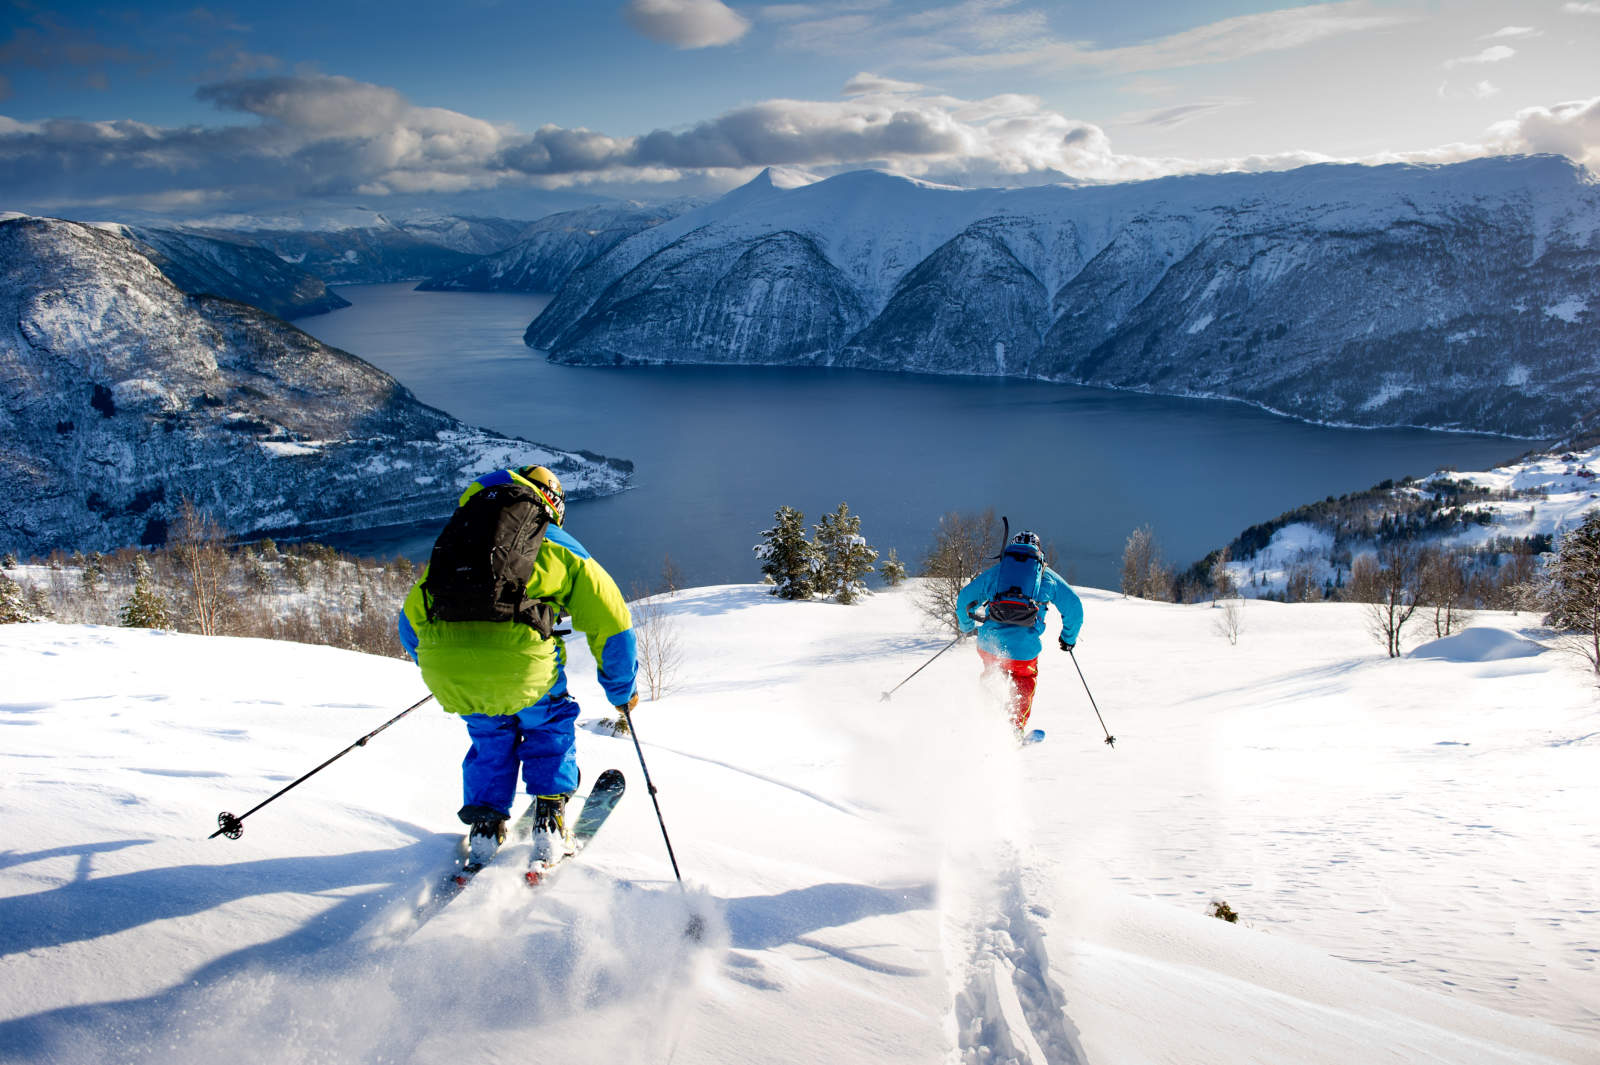
\includegraphics[height=\paperheight]{downhill}}
\begin{frame}[plain]
\end{frame}
\egroup

\begin{frame}[fragile]
  \frametitle{A descriptive approach}
  Firedrake, and FEniCS, mirror the mathematical abstraction of the
  finite element method in a \emph{domain specific language}.

  \begin{center}
\begin{minted}[fontsize=\tiny]{python}
V = FunctionSpace(mesh, "Lagrange", 1)
u = TrialFunction(V)
v = TestFunction(V)
a = inner(grad(u), grad(v))*dx
A = assemble(a)
\end{minted}
  \end{center}
  \begin{itemize}
  \item Symbolic description, implementation of ``maths'', not
    ``numerics''.
  \item Don't control everything, but did I need to?
  \end{itemize}
\end{frame}

\begin{frame}[fragile]
\begin{minted}[fontsize=\tiny]{c}
void cell_integral(double A[4][4], const double *const restrict *restrict coords) {
  static const double  t23[4]  = {-1.0, 0.0, 0.0, 1.0};
  static const double  t25[4]  = {-1.0, 0.0, 1.0, 0.0};
  static const double  t27[4]  = {-1.0, 1.0, 0.0, 0.0};
  ... /* Part of unrolled Jacobian computation */
  double t0  = (-1 * coords[0][0]);
  double t1  = (t0 + coords[1][0]);
  double t2  = (-1 * coords[0][1]);
  double t3  = (t2 + coords[2][1]);
  double t4  = (-1 * coords[0][2]);
  double t5  = (t4 + coords[3][2]);
  double t6  = (t2 + coords[3][1]);
  double t7  = (t4 + coords[2][2]);
  ...
  double t31  = (0.166666666666667 * fabs(t15));
  for (int k0 = 0; k0 < 4; k0++) {
    t28[k0] = ((t26 * t27[k0]) + (t24 * t25[k0])) + (t22 * t23[k0]);
    t29[k0] = ((t21 * t27[k0]) + (t20 * t25[k0])) + (t19 * t23[k0]);
    t30[k0] = ((t18 * t27[k0]) + (t17 * t25[k0])) + (t16 * t23[k0]);
  }
  for (int j0 = 0; j0 < 4; j0++) {
    double t32  = (((t26 * t27[j0]) + (t24 * t25[j0])) + (t22 * t23[j0]));
    double t33  = (((t21 * t27[j0]) + (t20 * t25[j0])) + (t19 * t23[j0]));
    double t34  = (((t18 * t27[j0]) + (t17 * t25[j0])) + (t16 * t23[j0]));
    for (int  k0  = 0; k0 < 4; k0 += 1) {
      A[j0][k0] += t31 * (((t34 * t30[k0]) + (t33 * t29[k0])) + (t32 * t28[k0]));
    }
  }
}
\end{minted}
\end{frame}

\begin{frame}
  \frametitle{A job for an expert}
  Hardware-aware optimsation of finite element kernels is a job for:
  \begin{itemize}
  \item<2-> A numerical analyst?
  \item<3-> A geodynamicist?
  \item<4-> A computational chemist?
  \item<5-> A computational scientist?
  \item<6-> A computer scientist?
  \end{itemize}
\end{frame}

\begin{frame}
  \frametitle{Form compilers}
  Translation of mathematical description of finite element problems
  carried out by a \emph{form compiler}.

  There are a few of these:

  \begin{itemize}
  \item DUNE: form compiler in development
  \item FFC: the FEniCS form compiler
  \item TSFC: the two stage form compiler
  \item SyFI: abandonware...
  \end{itemize}  
\end{frame}

\begin{frame}[fragile]
  \frametitle{Optimising compilers}
  \begin{itemize}
  \item Both code snippets are independent of polynomial degree.
    \emph{But}, the naive implementation is algorithmically
    suboptimal.

    \item \emph{Sum factorisation} (e.g. \textcite{Karniadakis:2005}) reduces
      operation count for residual evaluation from $\mathcal{O}(p^{2d})$
      to $\mathcal{O}(p^{d+1})$.
  \end{itemize}
  \begin{uncoverenv}<2>
    \begin{center}
\begin{minted}[fontsize=\tiny]{python}
V = FiniteElement("Lagrange", hexhedron, 7)
u = Coefficient(V)
v = TestFunction(V)
F = inner(grad(u), grad(v))*dx
count_flops(F, mode="vanilla") => 6668201
count_flops(F, mode="spectral") => 185257
\end{minted}
    \end{center}
  \end{uncoverenv}
\end{frame}

\begin{frame}
  \frametitle{Automating expertise}
  You can perform these optimisations by hand, but
  
  \begin{itemize}
  \item ``In-person'' case-by-case optimisation \emph{does not scale}
  \item Code generation allows us to package expertise and provide it
    to everyone
  \item Done by a domain compiler
  \item Anecdotally, research groups that have implemented ``high
    performance'' finite element code by hand, are now turning to
    domain compilers.
  \end{itemize}
\end{frame}

\section{Complex models}

\begin{frame}[fragile]
  \frametitle{Still fit on a slide!}
  \begin{columns}
    \begin{column}{0.48\framewidth}
      \begin{block}{Rayleigh-B\'enard convection}
        \small
        \begin{equation*}
          \begin{split}
            -\Delta u + u\cdot\nabla u + \nabla p +
            \frac{\text{Ra}}{\text{Pr}} \hat{g}T &= 0 \\
            \nabla \cdot u &= 0 \\
            - \frac{1}{\text{Pr}} \Delta T + u\cdot \nabla T &= 0
          \end{split}
        \end{equation*}
      \end{block}
    \end{column}
    \begin{column}{0.52\framewidth}
\begin{minted}[fontsize=\tiny,mathescape]{python}
from firedrake import *
mesh = Mesh(...)
V = VectorFunctionSpace(mesh, "CG", 2)
W = FunctionSpace(mesh, "CG", 1)
Q = FunctionSpace(mesh, "CG", 1)
Z = V * W * Q
upT = Function(Z)
u, p, T = split(upT)
v, q, S = TestFunctions(Z)
bcs = [...] # no-flow + temp gradient
nullspace = MixedVectorSpaceBasis(
   Z, [Z.sub(0), VectorSpaceBasis(constant=True), 
       Z.sub(2)])
F = (inner(grad(u), grad(v))
     + inner(dot(grad(u), u), v)
     - inner(p, div(v))
     + (Ra/Pr)*inner(T*g, v)
     + inner(div(u), q)
     + inner(dot(grad(T), u), S)
     + (1/Pr) * inner(grad(T), grad(S)))*dx

solve(F == 0, upT, bcs=bcs, nullspace=nullspace)
\end{minted}
    \end{column}
  \end{columns}
\end{frame}

\begin{frame}
  \frametitle{More than a pretty face}

  \begin{block}{Library usability}
    \begin{itemize}
    \item High-level language enables rapid model development
    \item Ease of experimentation
    \item Small model code base
    \end{itemize}
  \end{block}

  \begin{block}{Library development}
    \begin{itemize}
    \item Automation of complex optimisations
    \item Exploit expertise across disciplines
    \item Small library code base
    \end{itemize}
  \end{block}
\end{frame}

\begin{frame}
  \frametitle{Some questions to ask}
  Once I've set up my model, how much code do I have to change to:

  \begin{itemize}
  \item Change preconditioner?
  \item Drop terms in preconditioning operator?
  \item Use a different operator as preconditioner?
  \item Run quasi-Newton?
  \item Use matrix-free actions?
  \item Precondition matrix-free problems?
  \end{itemize}
\end{frame}

\begin{frame}
  \frametitle{Simple model development and experimentation}
  Fast prototyping is good, ``but I have to rewrite for performance''.

  \begin{itemize}
  \item Firedrake provides computational performance often >50\% achievable
    peak.
  \item Hero-coding necessary if you want the last 10-20\%
  \item ...but at what (person) cost?
  \end{itemize}  
\end{frame}

\begin{frame}
  \frametitle{Parallel ``for free''}
  \begin{itemize}
  \item Natural parallelisation is domain decomposition
  \item We can do this automatically given a mesh
  \item The mathematics doesn't say anything about parallelisation
  \item It's just a data parallel (``go do this everywhere'')
    description
  \item Model description says the same, so we can parallelise
    automatically
  \end{itemize}
\end{frame}

\begin{frame}
  \frametitle{Maintainability}
  \begin{columns}
    \begin{column}[t]{0.5\textwidth}
      \begin{block}{Core Firedrake}
        \begin{table}
          \centering
          \begin{tabular}{lc}
            Component & LOC   \\
            \hline
            Firedrake & 11500 \\
            PyOP2     & 6000  \\
            TSFC      & 3700  \\
            finat     & 600   \\
            \hline
            Total     & 21800
          \end{tabular}
        \end{table}
      \end{block}
    \end{column}
    \begin{column}[t]{0.5\textwidth}
      \begin{block}{Shared with FEniCS}
        \begin{table}
          \centering
          \begin{tabular}{lc}
            Component & LOC   \\
            \hline
            FIAT      & 4000  \\
            UFL       & 13000 \\
            \hline
            Total     & 17000
          \end{tabular}
        \end{table}        
      \end{block}
    \end{column}
  \end{columns}
\end{frame}

\begin{frame}
  \frametitle{Maintainable models}
  \begin{onlyenv}<1>
    \begin{block}{Thetis}
      \begin{center}
        \url{github.com/thetisproject/thetis}
      \end{center}
      \begin{itemize}
      \item 3D unstructured coastal ocean model written with Firedrake
      \item 6400 LOC
      \item 4x faster than previous code in group (same numerics)
      \end{itemize}
    \end{block}
  \end{onlyenv}
  \begin{onlyenv}<2>
    \begin{block}{Gusto}
      \begin{center}
        \url{www.firedrakeproject.org/gusto/}
      \end{center}
      \begin{itemize}
      \item 3D atmospheric dynamical core using compatible FE
      \item 1600 LOC
      \end{itemize}
    \end{block}
  \end{onlyenv}
\end{frame}

\begin{frame}[fragile]
  \frametitle{Automated manipulation of PDE solvers}
  \begin{block}{\url{www.dolfin-adjoint.org}}
    Automated derivation of the discrete adjoint from forward models
    written using FEniCS.

\begin{minted}[fontsize=\scriptsize]{sh}
$ cloc dolfin-adjoint/
Language  files   blank   comment   code
Python       52    2228       878   6939
$ cloc dolfin-adjoint/compatibility.py
Python        1      36         9    135
\end{minted}
  \end{block}  
\end{frame}

\section{Solving implicit systems}

\begin{frame}
  \frametitle{So I can write down a residual}
  \begin{itemize}
  \item It is easy to write down complex implicit systems.
  \item But the challenge is usually in solving them
  \item Firedrake provides access to PETSc for solving
  \item Any algebraic solver you like, plus composed fieldsplit solvers.
  \end{itemize}
\end{frame}

\begin{frame}
  \frametitle{Coupled problems make everything harder}
  \begin{itemize}
  \item Coupled problems are (typically) not amenable to black box solution
    methods.
  \item For small problems, can just use LU factorisation.
  \item For large problems, often use approximate block factorisations.
  \item Many configuration options, may require problem-specific
    auxiliary operators.
  \item Important to capture the abstraction so that automated model
    manipulation is still possible.
  \end{itemize}
\end{frame}

\begin{frame}
  \frametitle{Block preconditioning}
  Most state of the art preconditioning for multi-variable
  problems is based on block LU factorisations.

  \begin{uncoverenv}<2>
    \begin{equation*}
      T = \begin{bmatrix}
        A & 0 \\
        0 & C A^{-1} B^T
      \end{bmatrix}^{-1}
      \begin{bmatrix}
        A & B^T \\
        C & D = 0
      \end{bmatrix}
    \end{equation*}
    has minimal polynomial $T(T - I)(T^2 - T - I) =
    0$ \parencite{Murphy:2000}. \textcite{Ipsen:2001} treats case of
    $D \ne 0$.

    Alternate approach: ``function space''
    preconditioning \parencite{Kirby:2010,Mardal:2011,Malek:2014}.
  \end{uncoverenv}
\end{frame}

\begin{frame}[fragile]
  \frametitle{Rayleigh-B\'enard convection}

  \begin{columns}
    \begin{column}{0.48\framewidth}
        \small
        \begin{equation*}
          \begin{split}
            -\Delta u + u\cdot\nabla u + \nabla p +
            \frac{\text{Ra}}{\text{Pr}} \hat{g}T &= 0 \\
            \nabla \cdot u &= 0 \\
            - \frac{1}{\text{Pr}} \Delta T + u\cdot \nabla T &= 0
          \end{split}
        \end{equation*}
    \end{column}
    \begin{column}{0.52\framewidth}
  Newton updates need inverse of Jacobian:
  \begin{equation*}
    J = \begin{bmatrix}
      F   & B^T & M_1 \\
      C   & 0   & 0   \\
      M_2 & 0   & K
    \end{bmatrix}.
  \end{equation*}
  \begin{itemize}
  \item Navier-Stokes (top left)
  \item Convection-diffusion for temperature (bottom right)
  \item Coupling in $M_1$ and $M_2$ (non-symmetric).
  \end{itemize}
    \end{column}
  \end{columns}
\end{frame}
\begin{frame}
  \frametitle{Preconditioning}
  We will invert $J$ with a Krylov method, so we need a
  preconditioner.
  Let
  \begin{equation*}
    N = \begin{bmatrix}
      F & B^T\\
      C & 0 \\
    \end{bmatrix} \quad
    \tilde{M}_1 =
    \begin{bmatrix}
      M_1 \\
      0
    \end{bmatrix} \quad
    \tilde{M}_2 = \begin{bmatrix}
      M_2 & 0
    \end{bmatrix}
  \end{equation*}
  and block eliminate $N$ in $J$, giving system for temperature:
  \begin{equation*}
    S_T = K - \tilde{M}_2 N^{-1} \tilde{M}_1.
  \end{equation*}
  \textcite{Howle:2012} show that $K^{-1}$ is a good preconditioner for
  $S_T$.
\end{frame}
\begin{frame}
  \frametitle{Newton update}
  Solve for the update
  \begin{equation*}
    \begin{split}
      \delta x &= J^{-1} F(x). \\
      x &\leftarrow x + \delta x
    \end{split}
  \end{equation*}

  Write $\mathcal{K}(J, \mathbb{J})$ to denote approximating $J^{-1}$
  using an iteration $\mathcal{K}$ on $J$ using $\mathbb{J}$ as a
  preconditioner.  Then the iteration
  \begin{equation*}
    \KSP{J}{\begin{bmatrix}
      \ksp{N} & 0 \\
      0 & I
    \end{bmatrix}
    \begin{bmatrix}
      I & -\tilde{M}_1 \\
      0 & I
    \end{bmatrix}
    \begin{bmatrix}
      I & 0\\
      0 & \ksp{K}
    \end{bmatrix}}
  \end{equation*}
  empirically converges swiftly, and
  requires only $\mathbb{N}$ and $\mathbb{K}$.
\end{frame}

\begin{frame}
  \frametitle{Navier-Stokes block \parencite{Elman:2014}}
  A lower Schur complement factorisation of $N$ is a good option.
  Requires $\ksp{F}$ and $\KSP{S_p}{S}$ where $S_p = -C F^{-1} B^T$.

  One option is the \emph{pressure convection-diffusion}
  approximation:
  \begin{equation*}
    \mathbb{S} = \KSP{L_p}{L} F_p \KSP{M_p}{M},
  \end{equation*}
  so our recipe for $\ksp{N}$ is:
  \begin{equation*}
    \mathcal{K}\left(N, \begin{bmatrix}
      F & 0 \\
      0 & \mathcal{K}(S_p, \KSP{L_p}{L}\,F_p \, \KSP{M_p}{M})
    \end{bmatrix}
    \begin{bmatrix}
      I & 0\\
      -C & I
    \end{bmatrix}
    \begin{bmatrix}
      \ksp{F} & 0 \\
      0 & I
    \end{bmatrix}\right).
  \end{equation*}

\end{frame}

\begin{frame}
  \frametitle{Things to note}

  \begin{itemize}
  \item We only ever need inverses of diagonal blocks.
  \item Can save memory by applying operators matrix-free.
  \item The inverses are nested, we need ways of controlling the inner
    iterations.
  \end{itemize}

  \begin{block}{PCD}
    Needs the auxiliary discretised operator $F_p$ and approximate
    inverses of the auxiliary operators $L_p$ and $M_p$.

    Communication between PDE and solver libraries can no longer be
    \emph{unidirectional}.
  \end{block}
\end{frame}

\begin{frame}
  \frametitle{Firedrake \& PETSc to the rescue}
  \begin{itemize}
  \item PETSc already provides a highly runtime-configurable library
    for \emph{algebraically} composing solvers \parencite{Brown:2012}.

  \item Firedrake makes it straightforward to build auxiliary
    operators.

  \item We combine these to allow simple development of complex
    preconditioners.
  \end{itemize}
\end{frame}

\begin{frame}
  \frametitle{Two new pieces}
 
  \begin{onlyenv}<1>
    \begin{block}{A new matrix type}
      A PETSc shell matrix that implements matrix-free actions using
      Firedrake, and contains the UFL of the bilinear form.
    \end{block}
    
    \begin{block}{Custom preconditioners}
      These matrices do not have entries, so we create custom
      preconditioners that can inspect the UFL and do the appropriate
      thing.
    \end{block}
  \end{onlyenv}
  % \begin{onlyenv}<2>
  %   \begin{center}
  %     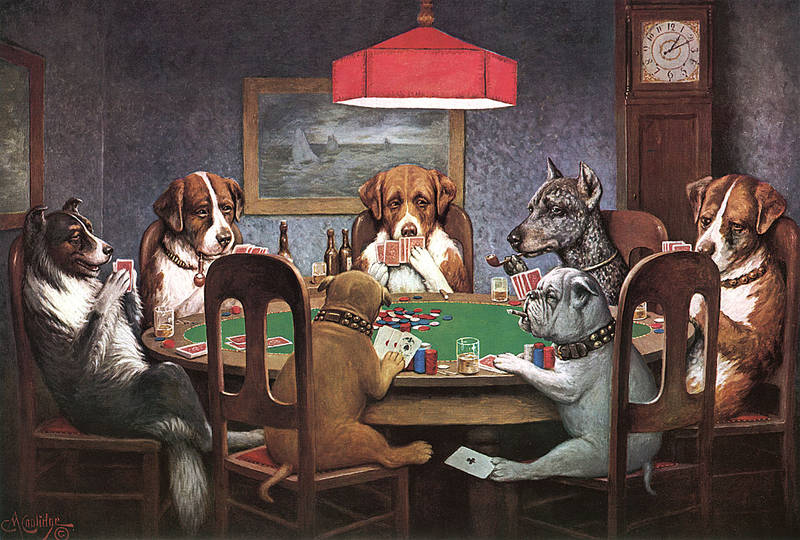
\includegraphics[width=0.8\textwidth]{underhand}
  %   \end{center}
  % \end{onlyenv}
\end{frame}

\begin{frame}[fragile]
  \frametitle{PCD}
\begin{minted}[fontsize=\tiny,mathescape]{python}
class PCDPC(PCBase):
    def initialize(self, pc):
        _, P = pc.getOperators()
        ctx = P.getContext()
        appctx = ctx.appctx
        p, q = ctx.arguments()
        [...] # Handling of boundary conditions elided
        M_p = assemble(p*q*dx)
        L_p = assemble(inner(grad(p), grad(q))*dx
        M_ksp = KSP().create()
        M_ksp.setOperators(M_p)
        L_ksp = KSP().create()
        L_ksp.setOperators(L_p)
        [...] # Some boilerplate elided
        u0 = split(appctx["state"])[appctx["velocity_space"]]
        F_p = assemble(inner(grad(p), grad(q))*dx + inner(u0, grad(p))*q*dx)

    def apply(self, pc, x, y):
        # $y \leftarrow \KSP{L_p}{L} F_p \KSP{M_p}{M} x$
        a, b = self.workspace
        self.M_ksp.solve(x, a)
        self.F_p.mult(a, b)
        self.L_ksp.solve(b, y)
\end{minted}
\end{frame}

\begin{frame}
  \frametitle{How to configure things}

  PETSc provides a ``programming language'' for configuring objects at
  runtime.  It has two operations

  \begin{enumerate}
  \item Value assignment
  \item String concatenation
  \end{enumerate}

  Every object has an \emph{options prefix} which controls where in
  the options database it looks for configuration values.

  This is verbose, but a very powerful idea.  We can control the types
  of individual solves by ensuring that they have different prefixes.
\end{frame}

\begin{frame}
  \frametitle{Back to the main event}
  We are solving
  \begin{equation*}
    \KSP{\begin{bmatrix}
        F & B^T & M_1\\
        C & 0 & 0 \\
        M_2 & 0 & K
      \end{bmatrix}}{J}
  \end{equation*}
  using
  \begin{equation*}
    \mathbb{J} =
    \begin{bmatrix}
      \KSP{\begin{bmatrix}
          F & B^T\\
          C & 0
        \end{bmatrix}}{N} & 0\\
      0 & I
    \end{bmatrix}
    \begin{bmatrix}
      I & 0 & -M_1\\
      0 & I & 0 \\
      0 & 0 & I
    \end{bmatrix}
    \begin{bmatrix}
      I & 0 & 0\\
      0 & I & 0\\
      0 & 0 &\ksp{K}
    \end{bmatrix}
  \end{equation*}
  with
  \begin{equation*}
    \mathbb{N} = \begin{bmatrix}
      F & 0 \\
      0 & \mathcal{K}(S_p, \KSP{L_p}{L}\,F_p \, \KSP{M_p}{M})
    \end{bmatrix}
    \begin{bmatrix}
      I & 0\\
      -C & I
    \end{bmatrix}
    \begin{bmatrix}
      \ksp{F} & 0 \\
      0 & I
    \end{bmatrix}
  \end{equation*}
  and
  \begin{equation*}
    S_p = -C \ksp{F} B^T.
  \end{equation*}
\end{frame}

\begin{frame}[fragile]
  \frametitle{Let's configure the Navier-Stokes solve}
  \small
  \begin{onlyenv}<1>
    \begin{equation*}
      \KSP{N}{%
        \begin{bmatrix}
          F & 0 \\
          0 & \mathcal{K}(S_p, \KSP{L_p}{L}\,F_p \, \KSP{M_p}{M})
        \end{bmatrix}
        \begin{bmatrix}
          I & 0\\
          -C & I
        \end{bmatrix}
        \begin{bmatrix}
          \ksp{F} & 0 \\
          0 & I
        \end{bmatrix}}
    \end{equation*}
\begin{minted}[fontsize=\tiny,escapeinside=||]{py}
-fieldsplit_0_ksp_type gmres
-fieldsplit_0_pc_type fieldsplit
-fieldsplit_0_pc_fieldsplit_type schur
-fieldsplit_0_pc_fieldsplit_schur_fact_type lower
-fieldsplit_0_fieldsplit_0_ksp_type preonly
-fieldsplit_0_fieldsplit_0_pc_type python
-fieldsplit_0_fieldsplit_0_pc_python_type firedrake.AssembledPC
-fieldsplit_0_fieldsplit_0_assembled_pc_type hypre
-fieldsplit_0_fieldsplit_1_ksp_type preonly
-fieldsplit_0_fieldsplit_1_pc_type python
-fieldsplit_0_fieldsplit_1_pc_python_type firedrake.PCDPC
-fieldsplit_0_fieldsplit_1_pcd_Fp_mat_type matfree
-fieldsplit_0_fieldsplit_1_pcd_Mp_ksp_type preonly
-fieldsplit_0_fieldsplit_1_pcd_Mp_pc_type ilu
-fieldsplit_0_fieldsplit_1_pcd_Kp_ksp_type preonly
-fieldsplit_0_fieldsplit_1_pcd_Kp_pc_type hypre
\end{minted}
  \end{onlyenv}
  \begin{onlyenv}<2>
    \color{gray}
    \begin{equation*}
      \highlight{$\mathcal{K}$}\left(N,%
        \begin{bmatrix}
        F & 0 \\
        0 & \mathcal{K}(S_p, \KSP{L_p}{L}\,F_p \, \KSP{M_p}{M})
      \end{bmatrix}
      \begin{bmatrix}
        I & 0\\
        -C & I
      \end{bmatrix}
      \begin{bmatrix}
        \ksp{F} & 0 \\
        0 & I
      \end{bmatrix}\right)
    \end{equation*}
\begin{minted}[fontsize=\tiny,escapeinside=||]{py}
|\highlight{-fieldsplit\_0\_ksp\_type gmres}|
-fieldsplit_0_pc_type fieldsplit
-fieldsplit_0_pc_fieldsplit_type schur
-fieldsplit_0_pc_fieldsplit_schur_fact_type lower
-fieldsplit_0_fieldsplit_0_ksp_type preonly
-fieldsplit_0_fieldsplit_0_pc_type python
-fieldsplit_0_fieldsplit_0_pc_python_type firedrake.AssembledPC
-fieldsplit_0_fieldsplit_0_assembled_pc_type hypre
-fieldsplit_0_fieldsplit_1_ksp_type preonly
-fieldsplit_0_fieldsplit_1_pc_type python
-fieldsplit_0_fieldsplit_1_pc_python_type firedrake.PCDPC
-fieldsplit_0_fieldsplit_1_pcd_Fp_mat_type matfree
-fieldsplit_0_fieldsplit_1_pcd_Mp_ksp_type preonly
-fieldsplit_0_fieldsplit_1_pcd_Mp_pc_type ilu
-fieldsplit_0_fieldsplit_1_pcd_Kp_ksp_type preonly
-fieldsplit_0_fieldsplit_1_pcd_Kp_pc_type hypre
\end{minted}
  \end{onlyenv}
  \begin{onlyenv}<3>
    \color{gray}
    \begin{equation*}
      \KSP{N}{%
        \highlight{$\begin{bmatrix}
        F & 0 \\
        0 & \mathcal{K}(S_p, \KSP{L_p}{L}\,F_p \, \KSP{M_p}{M})
      \end{bmatrix}
      \begin{bmatrix}
        I & 0\\
        -C & I
      \end{bmatrix}
      \begin{bmatrix}
        \ksp{F} & 0 \\
        0 & I
      \end{bmatrix}$}}
    \end{equation*}
\begin{minted}[fontsize=\tiny,escapeinside=||]{py}
-fieldsplit_0_ksp_type gmres
|\highlight{-fieldsplit\_0\_pc\_type fieldsplit}|
|\highlight{-fieldsplit\_0\_pc\_fieldsplit\_type schur}|
|\highlight{-fieldsplit\_0\_pc\_fieldsplit\_schur\_fact\_type lower}|
-fieldsplit_0_fieldsplit_0_ksp_type preonly
-fieldsplit_0_fieldsplit_0_pc_type python
-fieldsplit_0_fieldsplit_0_pc_python_type firedrake.AssembledPC
-fieldsplit_0_fieldsplit_0_assembled_pc_type hypre
-fieldsplit_0_fieldsplit_1_ksp_type preonly
-fieldsplit_0_fieldsplit_1_pc_type python
-fieldsplit_0_fieldsplit_1_pc_python_type firedrake.PCDPC
-fieldsplit_0_fieldsplit_1_pcd_Fp_mat_type matfree
-fieldsplit_0_fieldsplit_1_pcd_Mp_ksp_type preonly
-fieldsplit_0_fieldsplit_1_pcd_Mp_pc_type ilu
-fieldsplit_0_fieldsplit_1_pcd_Kp_ksp_type preonly
-fieldsplit_0_fieldsplit_1_pcd_Kp_pc_type hypre
\end{minted}
  \end{onlyenv}
  \begin{onlyenv}<4>
    \color{gray}
    \begin{equation*}
      \KSP{N}{%
        \begin{bmatrix}
        F & 0 \\
        0 & \mathcal{K}(S_p, \KSP{L_p}{L}\,F_p \, \KSP{M_p}{M})
      \end{bmatrix}
      \begin{bmatrix}
        I & 0\\
        -C & I
      \end{bmatrix}
      \begin{bmatrix}
        \highlight{$\mathcal{K}$}(K, \mathbb{K}) & 0 \\
        0 & I
      \end{bmatrix}}
    \end{equation*}
\begin{minted}[fontsize=\tiny,escapeinside=||]{py}
-fieldsplit_0_ksp_type gmres
-fieldsplit_0_pc_type fieldsplit
-fieldsplit_0_pc_fieldsplit_type schur
-fieldsplit_0_pc_fieldsplit_schur_fact_type lower
|\highlight{-fieldsplit\_0\_fieldsplit\_0\_ksp\_type preonly}|
-fieldsplit_0_fieldsplit_0_pc_type python
-fieldsplit_0_fieldsplit_0_pc_python_type firedrake.AssembledPC
-fieldsplit_0_fieldsplit_0_assembled_pc_type hypre
-fieldsplit_0_fieldsplit_1_ksp_type preonly
-fieldsplit_0_fieldsplit_1_pc_type python
-fieldsplit_0_fieldsplit_1_pc_python_type firedrake.PCDPC
-fieldsplit_0_fieldsplit_1_pcd_Fp_mat_type matfree
-fieldsplit_0_fieldsplit_1_pcd_Mp_ksp_type preonly
-fieldsplit_0_fieldsplit_1_pcd_Mp_pc_type ilu
-fieldsplit_0_fieldsplit_1_pcd_Kp_ksp_type preonly
-fieldsplit_0_fieldsplit_1_pcd_Kp_pc_type hypre
\end{minted}
  \end{onlyenv}
  \begin{onlyenv}<5>
    \color{gray}
    \begin{equation*}
      \KSP{N}{%
        \begin{bmatrix}
        F & 0 \\
        0 & \mathcal{K}(S_p, \KSP{L_p}{L}\,F_p \, \KSP{M_p}{M})
      \end{bmatrix}
      \begin{bmatrix}
        I & 0\\
        -C & I
      \end{bmatrix}
      \begin{bmatrix}
        \mathcal{K}(F, \highlight{$\mathbb{F}$}) & 0 \\
        0 & I
      \end{bmatrix}}
    \end{equation*}
\begin{minted}[fontsize=\tiny,escapeinside=||]{py}
-fieldsplit_0_ksp_type gmres
-fieldsplit_0_pc_type fieldsplit
-fieldsplit_0_pc_fieldsplit_type schur
-fieldsplit_0_pc_fieldsplit_schur_fact_type lower
-fieldsplit_0_fieldsplit_0_ksp_type preonly
|\highlight{-fieldsplit\_0\_fieldsplit\_0\_pc\_type python}|
|\highlight{-fieldsplit\_0\_fieldsplit\_0\_pc\_python\_type firedrake.AssembledPC}|
|\highlight{-fieldsplit\_0\_fieldsplit\_0\_assembled\_pc\_type hypre}|
-fieldsplit_0_fieldsplit_1_ksp_type preonly
-fieldsplit_0_fieldsplit_1_pc_type python
-fieldsplit_0_fieldsplit_1_pc_python_type firedrake.PCDPC
-fieldsplit_0_fieldsplit_1_pcd_Fp_mat_type matfree
-fieldsplit_0_fieldsplit_1_pcd_Mp_ksp_type preonly
-fieldsplit_0_fieldsplit_1_pcd_Mp_pc_type ilu
-fieldsplit_0_fieldsplit_1_pcd_Kp_ksp_type preonly
-fieldsplit_0_fieldsplit_1_pcd_Kp_pc_type hypre
\end{minted}
  \end{onlyenv}
  \begin{onlyenv}<6>
    \color{gray}
    \begin{equation*}
      \KSP{N}{%
        \begin{bmatrix}
        F & 0 \\
        0 & \highlight{$\mathcal{K}$}(S_p, \KSP{L_p}{L}\,F_p \, \KSP{M_p}{M})
      \end{bmatrix}
      \begin{bmatrix}
        I & 0\\
        -C & I
      \end{bmatrix}
      \begin{bmatrix}
        \ksp{F} & 0 \\
        0 & I
      \end{bmatrix}}
    \end{equation*}
\begin{minted}[fontsize=\tiny,escapeinside=||]{py}
-fieldsplit_0_ksp_type gmres
-fieldsplit_0_pc_type fieldsplit
-fieldsplit_0_pc_fieldsplit_type schur
-fieldsplit_0_pc_fieldsplit_schur_fact_type lower
-fieldsplit_0_fieldsplit_0_ksp_type preonly
-fieldsplit_0_fieldsplit_0_pc_type python
-fieldsplit_0_fieldsplit_0_pc_python_type firedrake.AssembledPC
-fieldsplit_0_fieldsplit_0_assembled_pc_type hypre
|\highlight{-fieldsplit\_0\_fieldsplit\_1\_ksp\_type preonly}|
-fieldsplit_0_fieldsplit_1_pc_type python
-fieldsplit_0_fieldsplit_1_pc_python_type firedrake.PCDPC
-fieldsplit_0_fieldsplit_1_pcd_Fp_mat_type matfree
-fieldsplit_0_fieldsplit_1_pcd_Mp_ksp_type preonly
-fieldsplit_0_fieldsplit_1_pcd_Mp_pc_type ilu
-fieldsplit_0_fieldsplit_1_pcd_Kp_ksp_type preonly
-fieldsplit_0_fieldsplit_1_pcd_Kp_pc_type hypre
\end{minted}
  \end{onlyenv}
  \begin{onlyenv}<7>
    \color{gray}
    \begin{equation*}
      \KSP{N}{%
        \begin{bmatrix}
        F & 0 \\
        0 & \mathcal{K}(S_p, \highlight{$\KSP{L_p}{L}\,F_p \, \KSP{M_p}{M}$})
      \end{bmatrix}
      \begin{bmatrix}
        I & 0\\
        -C & I
      \end{bmatrix}
      \begin{bmatrix}
        \ksp{F} & 0 \\
        0 & I
      \end{bmatrix}}
    \end{equation*}
\begin{minted}[fontsize=\tiny,escapeinside=||]{py}
-fieldsplit_0_ksp_type gmres
-fieldsplit_0_pc_type fieldsplit
-fieldsplit_0_pc_fieldsplit_type schur
-fieldsplit_0_pc_fieldsplit_schur_fact_type lower
-fieldsplit_0_fieldsplit_0_ksp_type preonly
-fieldsplit_0_fieldsplit_0_pc_type python
-fieldsplit_0_fieldsplit_0_pc_python_type firedrake.AssembledPC
-fieldsplit_0_fieldsplit_0_assembled_pc_type hypre
-fieldsplit_0_fieldsplit_1_ksp_type preonly
|\highlight{-fieldsplit\_0\_fieldsplit\_1\_pc\_type python}|
|\highlight{-fieldsplit\_0\_fieldsplit\_1\_pc\_python\_type firedrake.PCDPC}|
-fieldsplit_0_fieldsplit_1_pcd_Fp_mat_type matfree
-fieldsplit_0_fieldsplit_1_pcd_Mp_ksp_type preonly
-fieldsplit_0_fieldsplit_1_pcd_Mp_pc_type ilu
-fieldsplit_0_fieldsplit_1_pcd_Kp_ksp_type preonly
-fieldsplit_0_fieldsplit_1_pcd_Kp_pc_type hypre
\end{minted}
  \end{onlyenv}
  \begin{onlyenv}<8>
    \color{gray}
    \begin{equation*}
      \KSP{N}{%
        \begin{bmatrix}
        F & 0 \\
        0 & \mathcal{K}(S_p, \KSP{L_p}{L}\,\highlight{$F_p$} \, \KSP{M_p}{M})
      \end{bmatrix}
      \begin{bmatrix}
        I & 0\\
        -C & I
      \end{bmatrix}
      \begin{bmatrix}
        \ksp{F} & 0 \\
        0 & I
      \end{bmatrix}}
    \end{equation*}
\begin{minted}[fontsize=\tiny,escapeinside=||]{py}
-fieldsplit_0_ksp_type gmres
-fieldsplit_0_pc_type fieldsplit
-fieldsplit_0_pc_fieldsplit_type schur
-fieldsplit_0_pc_fieldsplit_schur_fact_type lower
-fieldsplit_0_fieldsplit_0_ksp_type preonly
-fieldsplit_0_fieldsplit_0_pc_type python
-fieldsplit_0_fieldsplit_0_pc_python_type firedrake.AssembledPC
-fieldsplit_0_fieldsplit_0_assembled_pc_type hypre
-fieldsplit_0_fieldsplit_1_ksp_type preonly
-fieldsplit_0_fieldsplit_1_pc_type python
-fieldsplit_0_fieldsplit_1_pc_python_type firedrake.PCDPC
|\highlight{-fieldsplit\_0\_fieldsplit\_1\_pcd\_Fp\_mat\_type aij}|
-fieldsplit_0_fieldsplit_1_pcd_Mp_ksp_type preonly
-fieldsplit_0_fieldsplit_1_pcd_Mp_pc_type ilu
-fieldsplit_0_fieldsplit_1_pcd_Kp_ksp_type preonly
-fieldsplit_0_fieldsplit_1_pcd_Kp_pc_type hypre
\end{minted}
  \end{onlyenv}
  \begin{onlyenv}<9>
    \color{gray}
    \begin{equation*}
      \KSP{N}{%
      \begin{bmatrix}
        F & 0 \\
        0 & \mathcal{K}(S_p, \KSP{L_p}{L}\,F_p \, \highlight{$\mathcal{K}$}(M_p, \mathbb{M}))
      \end{bmatrix}
      \begin{bmatrix}
        I & 0\\
        -C & I
      \end{bmatrix}
      \begin{bmatrix}
        \ksp{F} & 0 \\
        0 & I
      \end{bmatrix}}
    \end{equation*}
\begin{minted}[fontsize=\tiny,escapeinside=||]{py}
-fieldsplit_0_ksp_type gmres
-fieldsplit_0_pc_type fieldsplit
-fieldsplit_0_pc_fieldsplit_type schur
-fieldsplit_0_pc_fieldsplit_schur_fact_type lower
-fieldsplit_0_fieldsplit_0_ksp_type preonly
-fieldsplit_0_fieldsplit_0_pc_type python
-fieldsplit_0_fieldsplit_0_pc_python_type firedrake.AssembledPC
-fieldsplit_0_fieldsplit_0_assembled_pc_type hypre
-fieldsplit_0_fieldsplit_1_ksp_type preonly
-fieldsplit_0_fieldsplit_1_pc_type python
-fieldsplit_0_fieldsplit_1_pc_python_type firedrake.PCDPC
-fieldsplit_0_fieldsplit_1_pcd_Fp_mat_type matfree
|\highlight{-fieldsplit\_0\_fieldsplit\_1\_pcd\_Mp\_ksp\_type preonly}|
-fieldsplit_0_fieldsplit_1_pcd_Mp_pc_type ilu
-fieldsplit_0_fieldsplit_1_pcd_Kp_ksp_type preonly
-fieldsplit_0_fieldsplit_1_pcd_Kp_pc_type hypre
\end{minted}
  \end{onlyenv}
  \begin{onlyenv}<10>
    \color{gray}
    \begin{equation*}
      \KSP{N}{%
        \begin{bmatrix}
        F & 0 \\
        0 & \mathcal{K}(S_p, \KSP{L_p}{L}\,F_p \, \mathcal{K}(M_p, \highlight{$\mathbb{M}$}))
      \end{bmatrix}
      \begin{bmatrix}
        I & 0\\
        -C & I
      \end{bmatrix}
      \begin{bmatrix}
        \ksp{F} & 0 \\
        0 & I
      \end{bmatrix}}
    \end{equation*}
\begin{minted}[fontsize=\tiny,escapeinside=||]{py}
-fieldsplit_0_ksp_type gmres
-fieldsplit_0_pc_type fieldsplit
-fieldsplit_0_pc_fieldsplit_type schur
-fieldsplit_0_pc_fieldsplit_schur_fact_type lower
-fieldsplit_0_fieldsplit_0_ksp_type preonly
-fieldsplit_0_fieldsplit_0_pc_type python
-fieldsplit_0_fieldsplit_0_pc_python_type firedrake.AssembledPC
-fieldsplit_0_fieldsplit_0_assembled_pc_type hypre
-fieldsplit_0_fieldsplit_1_ksp_type preonly
-fieldsplit_0_fieldsplit_1_pc_type python
-fieldsplit_0_fieldsplit_1_pc_python_type firedrake.PCDPC
-fieldsplit_0_fieldsplit_1_pcd_Fp_mat_type matfree
-fieldsplit_0_fieldsplit_1_pcd_Mp_ksp_type preonly
|\highlight{-fieldsplit\_0\_fieldsplit\_1\_pcd\_Mp\_pc\_type ilu}|
-fieldsplit_0_fieldsplit_1_pcd_Kp_ksp_type preonly
-fieldsplit_0_fieldsplit_1_pcd_Kp_pc_type hypre
\end{minted}
  \end{onlyenv}
  \begin{onlyenv}<11>
    \color{gray}
    \begin{equation*}
      \KSP{N}{%
        \begin{bmatrix}
        F & 0 \\
        0 & \mathcal{K}(S_p, \highlight{$\mathcal{K}$}(L_p, \mathbb{L})\,F_p \, \KSP{M_p}{M})
      \end{bmatrix}
      \begin{bmatrix}
        I & 0\\
        -C & I
      \end{bmatrix}
      \begin{bmatrix}
        \ksp{F} & 0 \\
        0 & I
      \end{bmatrix}}
    \end{equation*}
\begin{minted}[fontsize=\tiny,escapeinside=||]{py}
-fieldsplit_0_ksp_type gmres
-fieldsplit_0_pc_type fieldsplit
-fieldsplit_0_pc_fieldsplit_type schur
-fieldsplit_0_pc_fieldsplit_schur_fact_type lower
-fieldsplit_0_fieldsplit_0_ksp_type preonly
-fieldsplit_0_fieldsplit_0_pc_type python
-fieldsplit_0_fieldsplit_0_pc_python_type firedrake.AssembledPC
-fieldsplit_0_fieldsplit_0_assembled_pc_type hypre
-fieldsplit_0_fieldsplit_1_ksp_type preonly
-fieldsplit_0_fieldsplit_1_pc_type python
-fieldsplit_0_fieldsplit_1_pc_python_type firedrake.PCDPC
-fieldsplit_0_fieldsplit_1_pcd_Fp_mat_type matfree
-fieldsplit_0_fieldsplit_1_pcd_Mp_ksp_type preonly
-fieldsplit_0_fieldsplit_1_pcd_Mp_pc_type ilu
|\highlight{-fieldsplit\_0\_fieldsplit\_1\_pcd\_Kp\_ksp\_type preonly}|
-fieldsplit_0_fieldsplit_1_pcd_Kp_pc_type hypre
\end{minted}
  \end{onlyenv}
  \begin{onlyenv}<12>
    \color{gray}
    \begin{equation*}
      \KSP{N}{%
        \begin{bmatrix}
        F & 0 \\
        0 & \mathcal{K}(S_p, \mathcal{K}(L_p, \highlight{$\mathbb{L}$})\,F_p \, \KSP{M_p}{M})
      \end{bmatrix}
      \begin{bmatrix}
        I & 0\\
        -C & I
      \end{bmatrix}
      \begin{bmatrix}
        \ksp{F} & 0 \\
        0 & I
      \end{bmatrix}}
    \end{equation*}
\begin{minted}[fontsize=\tiny,escapeinside=||]{py}
-fieldsplit_0_ksp_type gmres
-fieldsplit_0_pc_type fieldsplit
-fieldsplit_0_pc_fieldsplit_type schur
-fieldsplit_0_pc_fieldsplit_schur_fact_type lower
-fieldsplit_0_fieldsplit_0_ksp_type preonly
-fieldsplit_0_fieldsplit_0_pc_type python
-fieldsplit_0_fieldsplit_0_pc_python_type firedrake.AssembledPC
-fieldsplit_0_fieldsplit_0_assembled_pc_type hypre
-fieldsplit_0_fieldsplit_1_ksp_type preonly
-fieldsplit_0_fieldsplit_1_pc_type python
-fieldsplit_0_fieldsplit_1_pc_python_type firedrake.PCDPC
-fieldsplit_0_fieldsplit_1_pcd_Fp_mat_type matfree
-fieldsplit_0_fieldsplit_1_pcd_Mp_ksp_type preonly
-fieldsplit_0_fieldsplit_1_pcd_Mp_pc_type ilu
-fieldsplit_0_fieldsplit_1_pcd_Kp_ksp_type preonly
|\highlight{-fieldsplit\_0\_fieldsplit\_1\_pcd\_Kp\_pc\_type hypre}|
\end{minted}
  \end{onlyenv}
\end{frame}

\begin{frame}
  \frametitle{Runtime composability}

  \begin{itemize}
  \item Can tune implicit solve for Navier-Stokes on its own, then
    drop in where-ever such a block wants inverted.

  \item Model formulation doesn't care about variable
    splittings. Maybe we wanted to eliminate temperature first.  Do
    so, without changing the code.

  \item Composes with nonlinear solvers that need linearisations.

  \item Automatically take advantage of any improvements in Firedrake
    (fast matrix actions, etc...)

  \item No need to worry about parallel!
  \end{itemize}
\end{frame}

\begin{frame}
  \frametitle{Answering some questions}
  Once I've set up my model, how much code do I have to change to:

  \begin{itemize}
  \item Change preconditioner? 1-10 lines
  \item Drop terms in preconditioning operator? 1-10 lines
  \item Use a different operator as preconditioner? 1-10 lines
  \item Run quasi-Newton? 1-10 lines
  \item Use matrix-free actions? 1-10 lines
  \item Precondition matrix-free problems? 10-100 lines
  \end{itemize}
\end{frame}

\begin{frame}
  \frametitle{Open challenges}
  \begin{itemize}
  \item I haven't said anything about timestepping

  \item Problem, I think, is that there is no clean mathematical
    abstraction that captures a large enough class of methods.

  \item Some formulations (e.g. space-time DG) are amenable, but
    no-one has done the work.
    
  \item A challenge!
  \end{itemize}
\end{frame}


\appendix
\begin{frame}[t,allowframebreaks]
  \frametitle{References}
  \printbibliography[heading=none]
\end{frame}

\end{document}
